\documentclass[11pt]{article}

%\usepackage{palatino}

\usepackage[utf8]{inputenc}
\usepackage[T1]{fontenc}
\usepackage[sfdefault,scaled=.85]{FiraSans}
\usepackage{newtxsf}
\usepackage[spanish]{babel}
\usepackage{amssymb}
\usepackage{amsmath}
\usepackage{wasysym}
\usepackage[x11names, rgb, html]{xcolor}
\usepackage{graphicx}
\usepackage{caption}
\usepackage{float}
\usepackage{adjustbox}
\usepackage{geometry}
\usepackage[scaled=.85]{FiraMono}
\usepackage{algpseudocode}
\usepackage{algorithm}
\usepackage{hyperref}
\usepackage{listingsutf8}

\hypersetup{
  % hidelinks = true,   % Oculta todos los enlaces.
  colorlinks = true,   % Muestra todos los enlaces, sin bordes alrededor.
  linkcolor={black},     % Color de enlaces genéricos
  citecolor={blue!70!black},   % Color de enlaces de referencias
  urlcolor={blue!70!black}     % Color de enlaces de URL
}

\geometry{left=3cm,right=3cm,top=3cm,bottom=3cm,headheight=1cm,headsep=0.5cm}

\setlength{\parindent}{0pt}

%%% COLORES

\definecolor{50}{HTML}{FFEBEE}
\definecolor{100}{HTML}{FFCDD2}
\definecolor{200}{HTML}{EF9A9A}
\definecolor{300}{HTML}{E57373}
\definecolor{400}{HTML}{EF5350}
\definecolor{500}{HTML}{F44336}
\definecolor{600}{HTML}{E53935}
\definecolor{700}{HTML}{D32F2F}
\definecolor{800}{HTML}{C62828}
\definecolor{900}{HTML}{B71C1C}

%% Colores de Solarized

\definecolor{sbase03}{HTML}{002B36}
\definecolor{sbase02}{HTML}{073642}
\definecolor{sbase01}{HTML}{586E75}
\definecolor{sbase00}{HTML}{657B83}
\definecolor{sbase0}{HTML}{839496}
\definecolor{sbase1}{HTML}{93A1A1}
\definecolor{sbase2}{HTML}{EEE8D5}
\definecolor{sbase3}{HTML}{FDF6E3}
\definecolor{syellow}{HTML}{B58900}
\definecolor{sorange}{HTML}{CB4B16}
\definecolor{sred}{HTML}{DC322F}
\definecolor{smagenta}{HTML}{D33682}
\definecolor{sviolet}{HTML}{6C71C4}
\definecolor{sblue}{HTML}{268BD2}
\definecolor{scyan}{HTML}{2AA198}
\definecolor{sgreen}{HTML}{859900}

%% Colores del documento

\definecolor{text}{RGB}{78,78,78}
\definecolor{accent}{RGB}{129, 26, 24}

%%% LISTINGS

%% Tildes

\lstset{
  inputencoding=utf8/latin1
}

\lstset{
  % How/what to match
   sensitive=false,
  % Border (above and below)
  frame=leftline,
  rulecolor=\color{300},
  framerule=2pt,
  % Line number
  numbers=left,
  % Extra margin on line (align with paragraph)
  xleftmargin=\parindent,
  % Put extra space under caption
  belowcaptionskip=1\baselineskip,
  % Colors
  % backgroundcolor=\color{sbase3},
  basicstyle=\footnotesize\ttfamily\color{sbase00},
  keywordstyle=\color{700},
  commentstyle=\color{300},
  stringstyle=\color{500},
  numberstyle=\color{500},
  %identifierstyle=\color{500},
  % Break long lines into multiple lines?
  breaklines=true,
  % Show a character for spaces?
  showstringspaces=false,
  tabsize=2,
  xleftmargin=0.7em,
}

\renewcommand{\lstlistingname}{Código fuente}% Listing -> Algorithm


\title{Sistemas Concurrentes y Distribuidos\\ \large El conjunto de Mandelbrot con MPI}
\author{Antonio Coín Castro}
\date{\today}

\begin{document}
\maketitle


\section*{El conjunto de Mandelbrot}

El conjunto de Mandelbrot es un \textit{conjunto fractal}, digamos $M$, definido en el plano complejo como sigue: un número $c$ pertene a $M$ si la sucesión $z_0 = 0, \ z_{n+1} = z_n^2 + c$ queda acotada, o equivalentemente, si $|z_n| \le 2$ sin importar lo grande que sea $n$. Para más información se puede consultar \cite{mandelbrot}.



\section*{Esquema de un algoritmo basado en paso de mensajes}

Con el objetivo de construir un algoritmo para dibujar el conjunto de Mandelbrot, empleamos la técnica de paso de mensajes en un esquema maestro-esclavo siguiendo la idea de la diapositiva 59 del tema 3 de la asignatura. \\

Como primera observación, notamos que trabajaremos en un rectángulo del plano complejo, el equivalente a $[-2,2] \times [-2,2]$. En este rectángulo, necesitaremos dividir los complejos en elementos discretos, para así poder convertirlos en píxeles y crear una imagen.\\

Un esquema del código del proceso maestro es el siguiente:

\begin{algorithm}[h]
\begin{algorithmic}

\Function{Maestro}{}
     
     \For{i $:=$ $0$ to $n_e-1$}
         \State send(fila, Esclavo[i]);
            \EndFor
         \While{\textit{quedan filas sin colorear}}
         	\State select
         	\For{j $:=$ $0$ to $n_e-1$ when receive(colores, Esclavo[j])}
         		\If {\textit{quedan filas sin mandar}}
         		\State send(fila, Esclavo[j]);
         		\Else
         		    \State send(fin, Esclavo[j]);
         		\EndIf
         	\EndFor
         \EndWhile
         \State visualiza(colores);
  \EndFunction
\end{algorithmic}
\end{algorithm}

Como vemos, el maestro se encarga de enviar a los esclavos filas completas de números complejos a demanda. Además, recibe las filas ya procesadas, y espera a completar el proceso para visualizar la imagen.\\

Los esclavos, por su parte, van recibiendo filas de complejos y las devuelven al maestro ya coloreadas mediante un cierto algoritmo:

\begin{algorithm}
\begin{algorithmic}
	\Function{Esclavo }{ $i : 0 \dots n_e-1$}
     \State receive(mensaje, Maestro);
     \While{mensaje $\ne$ fin}
        \State colores $:=$ calcula\_colores(mensaje.fila);
         \State send(colores, Maestro);
          \State receive(mensaje, Maestro);
     \EndWhile
    \EndFunction
\end{algorithmic}
\end{algorithm}

\section*{Implementación en C++ con MPI}

Para implementar el algoritmo en el lenguaje \verb|C++|, utilizamos la librería de paso de mensajes MPI. Para generar la imagen obtenida del conjunto de Mandelbrot empleamos la librería \verb|png++| \cite{png++}, que se trata de un \textit{wrapper} para la conocida librería \verb|libpng|. Procedemos ahora a analizar los puntos clave del programa, que puede encontrarse en el fichero \verb|mandelbrot.cpp|.


\subsection*{Convertir píxeles en números complejos}

Para transformar los píxeles de nuestra imagen en números complejos, realizamos un simple trabajo de discretización sobre el rectángulo definido. Aquí entra en juego la \textbf{precisión} (\textit{jump}) con la que queremos discretizar el campo complejo.
\vspace{0.5em}

\lstinputlisting[language=C++, linerange={65-73}]{./mandelbrot.cpp}

\subsection*{Proceso maestro}
El proceso maestro se comporta tal y como mostramos en el pseudocódigo, con la salvedad de que junto a cada fila envía un identificador de fila, para facilitar el proceso de reconstrucción de la imagen.
\vspace{0.5em}

\lstinputlisting[language=C++, linerange={164-193}]{./mandelbrot.cpp}

\subsection*{Proceso esclavo}
De nuevo, el esclavo funciona de forma muy similar a la mostrada anteriormente, teniendo en cuenta la restricción adicional de que en cada comunicación intervienen dos mensajes: un identificador de fila, y después el contenido de la misma.
\vspace{0.5em}

\lstinputlisting[language=C++, linerange={215-229}]{./mandelbrot.cpp}

\subsection*{Algoritmo de tiempo de escape}
Este algoritmo simplemente realiza iteraciones de la sucesión de Mandelbrot hasta un límite impuesto por el programador, y establece el color del píxel en cuestión en función del número de iteraciones realizadas. 
\vspace{0.5em}

\lstinputlisting[language=C++, linerange={111-121}]{./mandelbrot.cpp}

\vspace{0.5em}
Para decidir el color de cada píxel disponemos de dos algoritmos, conocimos como \textit{linear coloring} y \textit{continuous coloring}. En el primero pintamos de negro los puntos que consideramos que pertenecen al conjunto, mientras que los puntos que probablemente no pertenecen se van aclarando hasta llegar al blanco. Esto se consigue mediante un escalado de las iteraciones hasta los posibles valores de \verb|RGB| ($0$-$255$).
\vspace{0.5em}

\lstinputlisting[language=C++, linerange={124-126}]{./mandelbrot.cpp}

\vspace{0.5em}
En el segundo algoritmo, calculamos un número en el intervalo $[0,1)$, y lo multiplicamos por 255 para obtener el color final del píxel. De esta forma se consigue un espacio de colores continuo. La justificación del funcionamiento de  este algoritmo se puede consultar en \cite{mandelbrot_smooth}.
\vspace{0.5em}

\lstinputlisting[language=C++, linerange={128-139}]{./mandelbrot.cpp}

\subsection*{Mostrar la imagen final}

Para construir la imagen, identificamos cada complejo del rectángulo definido con un píxel coloreado, y en la orientación que nos interesa. Además, empleamos una escala para que la imagen resultante tenga siempre un tamaño fijo.
\vspace{0.5em}

\lstinputlisting[language=C++, linerange={83-98}]{./mandelbrot.cpp}

\vspace{0.5em}
La imagen resultante se guarda en el directiorio actual como \verb|mandelbrot.png|.

\section*{Resultados}
Por último, mostramos el resultado de una ejecución con precisión p=0.001. El tiempo de ejecución en mi máquina (Intel Core i5-7200U @ 2.5 GHz) es de unos 90 segundos. El tamaño de imagen elegido es 1024 $\times$ 1024, y el límite de iteraciones es 1000.\\

Este resultado es muy similar al obtenido con una precisión 10 veces mayor, que tarda en la misma máquina unos 110 minutos (supone evaluar casi 16 millones más de números complejos).

\begin{figure}[!ht]
    \centering
    
\includegraphics[width=.65\textwidth]{img/0001-cropped}
	\caption{Conjunto de Mandelbrot con coloreado lineal}
\end{figure}

\newpage

La misma ejecución con el algoritmo de coloreado continuo resulta en esta imagen:\\

\begin{figure}[!ht]
    \centering
    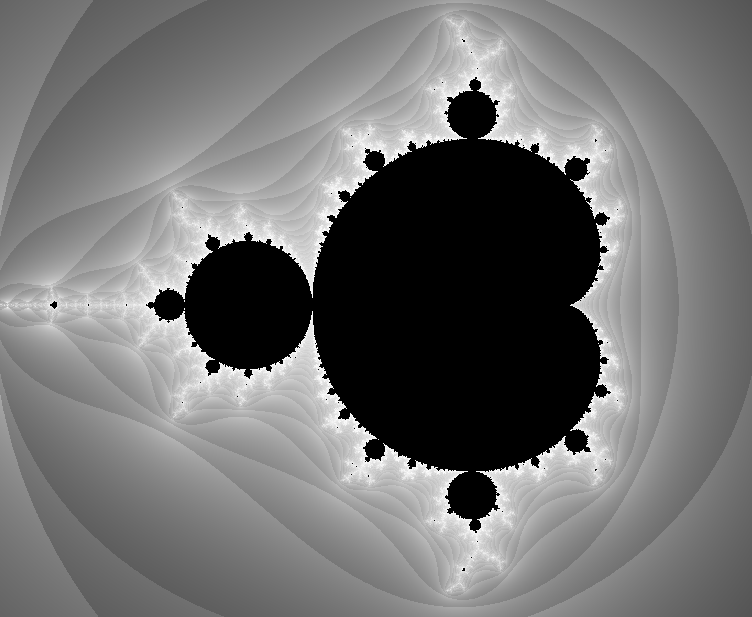
\includegraphics[width=.65\textwidth]{img/0001-smooth-cropped}
	\caption{Conjunto de Mandelbrot calculado con coloreado continuo}
\end{figure}


\section*{Compilación}

Se proporciona un \verb|makefile| para compilar y ejecutar el programa. Es necesario trabajar bajo un entorno \verb|Linux| y tener instalada las librerías \verb|libpng| y \verb|openMPI|.

% ---------------------------------------------------------------------------
% Bibliografía.
% ---------------------------------------------------------------------------
\begin{thebibliography}{9}

\bibitem{mandelbrot}
  Mandelbrot set on \href{https://en.wikipedia.org/wiki/Mandelbrot_set}{Wikipedia}.

\bibitem{png++} 
  Wrapper for libpng: \href{http://www.nongnu.org/pngpp/doc/0.2.9/index.html}{png++}.

\bibitem{mandelbrot_smooth} 
  \href{https://en.wikipedia.org/wiki/Mandelbrot_set#Continuous_(smooth)_coloring}{Continuous coloring algorithm}.

\end{thebibliography}


\end{document}
